%!TEX root = ../thesis.tex

\cleardoublepage
\chapter{Approach}
\label{cha:approach}


This chapter covers how a solution was integrated into a scientific workflow manager, as well as the specific parameters and reward functions of the reinforcement learning agents. In section \ref{sec:integration} the software architecture of the approach and its integration with the nextflow source code will be discussed, and then in \ref{sec:gradient_bandits} and \ref{sec:q_agent} respectively the details of the gradient bandit and the q-learning agents will be considered. 

%%=========================================
\section{Integrating a Solution into a Workflow Manager}
\label{sec:integration}

Nextflow \cite{nextflow} is a robust scientific workflow management system written primarily in groovy. It supports various execution platforms and has a large variety of tools to help users analyse the performance of their workflows. Nextflow is free open source software and for this thesis a fork of the 20.12.0 version was used \footnote{https://git.tu-berlin.de/zunkernicolas/nextflow-extension}. In order to integrate a reinforcement learning approach with the nextflow source code a simple structure was designed which externalised the storage of data from previous tasks and workflows so that when a task needed to be scheduled the reinforcement learning agent could retrieve historical data about the task from a database to inform its decision. The structure can be seen in the following figure.

\begin{figure}[ht]
    \centering
        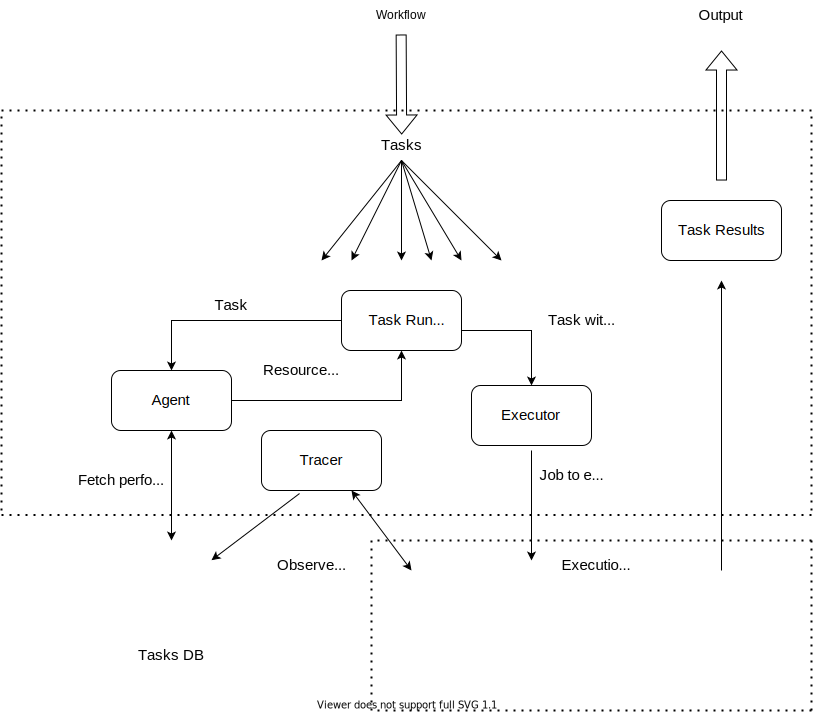
\includegraphics[width=0.8\textwidth]{fig/implementation_diagram.png}
        \caption{High Level Design: Integration of a Reinforcement-Learning Agent into Nextflow}
        \label{fig:implementation}
\end{figure}

Although the code for the reinforcement learning agents is logically a part of nextflow, when discussing the above design they will be referenced separately. The interaction between nextflow, the agents, and the external actors (the user, the database and the execution platform) is as follows. First, before a task is ready to be scheduled it is sent to a reinforcement-learning agent specific to that task, for the purposes of this thesis that was either a q-learning agent or a gradient bandit. Next, the task’s agent would then retrieve historical performance data and any other relevant data (i.e. what state the agent was last in) from the database. This database is external to nextflow and the creation and management of this database is not performed by nextflow or the agent which only use the database to save or read data beyond a workflow’s lifetime. Then, using the data, the agent selects a new resource allocation for the task and overwrites the task’s default configuration. After this, nextflow uses its custom executor for the given execution platform to prepare the task and pass it on to that platform. The task is then executed on the platform. It is important to note that the execution platform will also have its own system for managing, scheduling and executing jobs and processes. As the task is executed nextflow’s tracer module will gather performance data, i.e. peak CPU usage and peak RSS \footnote{https://www.nextflow.io/docs/}. Finally, once the task is finished all of this data is stored in the database for the agent to use the next time the task comes. It is important to note that there is one agent for each unique task. These agents are called whenever their task needs to be executed and they use the database to receive rewards for their previous actions.

Now that the structure of the agent’s environment has been explained and the relationship between collecting data and assigning a task resources is clear, it is time to delve into the specific approaches tried.

\section{Gradient Bandits}
\label{sec:gradient_bandits}

In the course of this thesis gradient bandits were used to allocate both CPUs and memory. The way they did this will be explained here.

\subsection{CPU Bandit}
\label{sub:cpu_bandit}

\subsubsection{Design}
\label{subsub:bandit1_design}

The CPU Bandit, as it was nicknamed, had a very simple set of actions to choose from which were based on the number of CPUs available to the system. The bandit then learned how many CPUs to allocate to its task. Its reward was a very straightforward function:

\begin{equation}
\label{bandit1_reward}
reward = -t\times(1+cpus - cpu\_usage/100)
\end{equation}


In this equation $cpu\_usage$ is a value in percent of the number of single core CPUs used by the task. If a task were assigned 4 CPUs and only effectively used two of them then $cpu\_usage$ would be $200$\%. $cpus$ is the number of CPUs assigned to the task and $t$ is how long the task took to run. Put in other words this equation punishes the agent with a negative reward equal to the amount of time it ran plus the unused CPU time (execution time multiplied by the number of unused CPUs). The idea is to provide an incentive for the agent to try to minimise the amount of time where any of the allocated CPU’s are not being used, and by punishing it with the amount of time that the task ran for, the agent is also encouraged to try to reduce the amount of time taken for the task to complete. This also means that, should a task have 100\% usage then its penalty is not 0 but is just the execution time. The reason for including time in the reward function is that if the agent has no concept of time it will always allocate the least amount of resources possible, since that is guaranteed to minimise the amount of resources wasted, and ultimately the tasks and their workflows would all be incredibly slow. 

\subsubsection{Picking the Right Step Size}
\label{subsub:const_stepsize}
The most pressing issue encountered with the CPU bandit approach was related to the step size. The initial step size $\alpha$ was $0.1$, which would be an appropriate step size for a bounded reward function with a mean reward that is around 10 or is known to have a standard deviation less than that (these values are based on the example given in \cite{sutton_barto} where they use a step size of 0.1 for a reward function with a statistical mean of 4). However the reward function used in \ref{bandit1_reward} has the bounds [ $-time \times (cpus+1)$ , $-time$ ] and as such is unbounded, since $time$ can be arbitrarily large and the standard deviation which was observed for the rewards was also too large. Therefore whenever tasks had a runtime $> 10$ seconds, $\alpha$ was too large. 

The danger in using a constant step size which is too large for the reward function is that when the bandit receives a reward which is considerably larger than the previous average the “step” taken in the direction of that action will also be too large and the bandits preferences will be updated such that the given action is always preferred and no other actions are tried any more. This causes the bandit to cease exploration too early. This effect was a common problem for tasks which took longer than 20 seconds to complete and was especially pronounced for tasks with runtimes of 100 seconds and more.  For these tasks the inherent volatility of the reward function relative to a step size of 0.1 meant that the bandits were converging very early and often had not explored the other actions at all. To provide a concrete example: if a bandit’s third allocation of CPUs received a reward of -150 and the first two allocations had had an average reward of -200, then for a step size of 0.1 the preference for the new allocation would increase by approximately $50\times0.1=5$. Now because of the exponential nature of the soft max distribution function used on the preferences, the probability of picking that action would increase by a large amount and then the bandit is in danger of converging to that allocation without any more exploration. This is best demonstrated graphically, as can be seen in figures \ref{fig:sub1} and \ref{fig:sub2}.

\begin{figure}[ht]
\centering
\begin{subfigure}{.5\textwidth}
  %\centering
  \includegraphics[width=\textwidth,height=\textwidth]{fig/old_UNICYCLER.png}
  \caption{Bandit 1}
  \label{fig:sub1}
\end{subfigure}%
\begin{subfigure}{.5\textwidth}
 % \centering
  \includegraphics[width=\textwidth,height=\textwidth]{fig/old_BOWTIE2.png}
  \caption{Bandit 2}
  \label{fig:sub2}
\end{subfigure}
\caption{Example of Two Bandits Converging Too Fast}
%\label{fig:old_bandits}
\end{figure}

These figures show two gradient bandits which were exhibiting the behaviour described above. Each figure is made up of 2 graphs which display the action chosen by the bandit in the top graph and the probabilities for all of the actions in the bottom graph. As can be seen in the two examples, after receiving a relatively large reward, the agent’s probability of choosing a given action rises far too quickly and no other actions are attempted thereafter. This is occurring because the step taken by the bandit in the direction of a single action’s preference is too large and the resulting probability of choosing that action grows so much that no other actions are explored any more. 

The solution to this problem is to adjust the step size so that it is not a constant value but is instead a function which uses the average time that it usually takes the task to complete. This way tasks which have longer average runtimes are given smaller step sizes. The new value for $\alpha$ is thus $1/avg(time)$.

\begin{figure}[ht]
\centering
\begin{subfigure}{.5\textwidth}
  %\centering
  \includegraphics[width=\textwidth,height=\textwidth]{fig/UNICYCLER.png}
  \caption{Bandit 1}
  \label{fig:sub3}
\end{subfigure}%
\begin{subfigure}{.5\textwidth}
 % \centering
  \includegraphics[width=\textwidth,height=\textwidth]{fig/BOWTIE2.png}
  \caption{Bandit 2}
  \label{fig:sub4}
\end{subfigure}
\caption{Bandits with a Step Size Based on Their Historical Average Execution Time}
\label{fig:fixed_bandits}
\end{figure}

The next two figures \ref{fig:sub3}, \ref{fig:sub4} show the same two tasks and their bandits but with the new step size. As can be seen the exploration phase is considerably longer and many different CPU allocations (actions) are tried before settling on one. Specifically in the case of the \textit{UNICYCLER} task’s bandit we can see that although allocating 3 CPUs seems to develop a strong preference early on (perhaps because it performed abnormally well once or perhaps because it genuinely is the best performing allocation) it does not become so preferred as to be dominant until much later and until that point the bandit continued to try other options.

It should be noted that these changes mean that for optimal performance of the bandits there should already be some historical data available about the task’s and their runtimes. It is not a necessity because over time the bandit can gather this data itself, but it is preferable.

\subsection{Memory Bandit}
\label{sub:mem_bandit}
The other gradient bandit approach used for assigning resources to tasks was called the memory bandit and its available actions were memory assignments. Beyond the obvious, the memory bandit was different from the CPU bandit in two respects. Firstly, the amount of memory available is several order of magnitudes larger than the amount of cpus. Thus, in order to limit the number of available actions to a manageable amount, the original amount of memory assigned to the task $m$ (in the default configuration) had to be split up into $n$ chunk,s each of size $c=m/n$. The bandit is then presented $a$ actions, each of which assigns $a\times c$ amounts of memory to the task. $a$ can be chosen as $1.5 \times n$ to give a good balance between considering allocations that are larger and smaller than the default configuration, however since it is known in advance that user estimates are usually quite poor one could also choose $a < n$ to encourage memory efficiency. In addition to this, by choosing larger or smaller $n$ values the size of the memory chunks can be adjusted. Secondly, and this is the biggest difference between the two bandits, a task which is assigned too little memory and overuses it will be killed. This means that there must be a special penalty for such cases.

The reward function used for the memory bandit, after assigning $memory$ bytes of memory is as follows:

\[ reward = 
\begin{cases}
   % \frac{x^2-x}{x},& \text{if } x\geq 1\\
    -2\times memory/c,& \text{if the task ran out of memory}\\
    -1 \times unused\_chunks              & \text{otherwise}
\end{cases}
\]

Where $unused\_chunks = (memory - peak\_rss) / c$ and $peak\_rss$ is the peak resident set size (RSS), in bytes, of the task during its execution.

An obvious alternative for this function is to simply use the memory usage: $reward = peak\_rss/mem$, and $\alpha = 0.01$ since the reward function’s range is [0,100]. However during testing this was found to be too small for tasks which have a low memory footprint. For example a task which uses 1\% of the assigned memory when assigned $n$ chunks, and thus receives a reward of 1\%, will only yield a maximum reward of $n$\% for the optimal allocation of just one memory chunk and for such small differences a gradient bandit will struggle to recognize the superior choice, even though it should be obvious. This is especially damaging to performance because these low usage tasks are precisely the ones where memory efficiency can be optimized the most and as such the reward function was changed to one which penalises the agent for the amount of unused memory. Of course to avoid the problem the CPU bandit had with its step size, the amount of unused memory in bytes could not be used and therefore the number of unused memory chunks was used instead. To return to the example of a task with 1\% usage that task’s rewards would now be $-n$ at worst and $-1$ at best, which makes it much easier for the bandit to determine good allocations. Finally in the case where a task has been killed the penalty is equal to double the number of memory chunks assigned because the agent must (at the very least) assign the same amount of memory again or must assign even more memory.

The actual implementation of the memory bandit is slightly adjusted so that whenever a task fails with one memory allocation and is retried with a new one, the new allocation must be greater than the previous one. If the bandit does pick a smaller allocation then it is ignored and the new allocation is either doubled or the default configuration for that task is used (if double the new allocation is also less than the failed allocation). This prevents the workflow from being broken off if a given task fails too many times due to repeated poor allocations.

Finally, to return to a discussion of step size similar to that in \ref{subsub:const_stepsize}, the memory bandit can be assigned a constant step size $\alpha = 1/n$. This is is because for $n$ memory chunks, the bandits reward function is bounded by [$-n$, 0]. 


\section{Q-learning Agent}
\label{sec:q_agent}

Similar to the approach with the gradient bandits, there was one q-learning agent per unique task. The q-learning agent’s state was always the current allocation of CPU and memory for the given task, and as its set of actions it could choose between incrementing or decrementing the amount of CPUs or memory, or it could do nothing. To limit the state space the maximum and minimum number of CPUs and memory as well as the amount by which they were incremented or decremented was based on the default allocation given to the task by the developers of the workflow (provided they did not exceed the resources of the execution platform). When the task was scheduled by the agent for the first time it would start in the default configuration’s state. Just like the memory bandit in section \ref{sub:mem_bandit} the possible memory states of the reinforcement learning agent are also chunks of memory. 

For the q-learning agent a different reward function was used than for the CPU bandit, primarily because it also had to incorporate memory but also as part of an attempt to experiment with different reward functions and approaches. 

\begin{equation}
\label{q_agent_1_reward}
r = -max(0.1,unused\_cpus) \times (t/avg\_t) \times (mem\times (1 - max(0.75,mem\_use)))
\end{equation}

Here the $mem$ variable refers to the memory allocated to the process and $mem\_use$ is the value of of the peak RSS of the task divided by the memory assigned to it. $avg\_t$ is a constant value which is determined at runtime based on the historical average execution time for the task. Lastly, $unused\_cpus = cpus - cpu\_usage/100$ where $cpus$ and $cpu\_usage$ are the same as in \ref{bandit1_reward}. 

Since division by the task’s average time is incorporated into the reward function it did not need to be incorporated into the step size as with the gradient bandit (see \ref{subsub:const_stepsize}) and the issues associated with that were avoided. This function is effectively a product of the number of unused CPUs, the slow-down factor and the amount of unused memory. However there are some slight modifications. The $max$ function is used to set an artificial floor for the penalty incurred by the unused CPUs and unused memory. Tasks which use more than 90\% of the available CPUs are given the same reward as tasks which use exactly 90\% in an attempt to prevent the agent from deciding to assign each task 1 CPU in order to minimise the number of unused CPUs. Additionally the floor for unused memory is capped at 25\% in a similar manner. This is done to discourage the agent from allocating too little memory because tasks which use too much memory will of course be killed and have to start over, which can have a detrimental effect on performance. This reward function is of course negated in order to turn it into a penalty function so that the agent will seek to minimise its penalty by minimising the number of unused CPUs, the slowdown and the amount of unused memory.

The q-learning agent also has 3 other parameters- the step size $\alpha$, epsilon $\epsilon$ and the discount $\gamma$. Step size was set to 0.1 and the discount was 1.0. Epsilon is adjusted over time- at first it is 0.5, to encourage exploration, then after 50 runs it is decreased to 0.25 and after 100 runs it is 0.1 to discourage exploration but leave room for the bandit to still occasionally try other actions and visit different states.

\subsubsection{Exploring the State-Action Space}
\label{subsub:states}

It should be noted here that unlike the gradient bandits from before, which had to decide from $c$ or $n$ number of actions for the CPU and memory bandits respectively, the q-learning agent must learn the value function for $(c-2)*((m-2)*a + 2*(a-1)) + 2*((m-2)*(a-1) + 2*(a-2))$ state-action combinations. Here $c$ is the number of possible CPU states, $m$ is the number of possible memory states and $a=5$ is the number of possible actions. Now since the q-learning algorithm from \ref{alg:q-learning} needs to try each action in every state combination at least once, and explores with probability $\epsilon$ then for arbitrary examples of $c=4$ and $m=3$ it will take, at the very least, 46 different runs just to have tried every action in every state once. This shows how much more complex the q-learning approach is than the gradient bandit approaches. Ultimately however the theoretical benefit posed by q-learning is that when the agent learns, for example, not to increment the amount of CPUs when in state $s$ (where $s$ is also the number of CPUs currently allocated), the agent is thus also learning to avoid all states/allocations $\{s_c \in S$ $|$ $s_c > s\}$ which allocate more CPUs than $s$. While this seems trivial, the gradient bandit is unable to see such connections and cannot tell that a task which has low CPU usage for $s$ CPUs can be expected to have even lower usage for $s_c > s$ CPUs. 


